\documentclass{classrep}
\usepackage[utf8]{inputenc}
\frenchspacing

\usepackage{graphicx}
\usepackage[usenames,dvipsnames]{color}
\usepackage[hidelinks]{hyperref}
\usepackage{lmodern}
\usepackage{graphicx}
\usepackage{placeins}
\usepackage{url}
\usepackage{amsmath, amssymb, mathtools}

\usepackage{fancyhdr, lastpage}
\pagestyle{fancyplain}
\fancyhf{}
\renewcommand{\headrulewidth}{0pt}
\cfoot{\thepage\ / \pageref*{LastPage}}


\studycycle{Informatyka, studia dzienne, I st.}
\coursesemester{IV}

\coursename{Inteligentna Analiza Danych}
\courseyear{2018/2019}

\courseteacher{mgr inż. Paweł Tarasiuk}
\coursegroup{poniedziałek, 12:15}

\author{%
  \studentinfo[216806@edu.p.lodz.pl]{Kamil Kowalewski}{216806}\\
  \studentinfo[216920@edu.p.lodz.pl]{Tomasz Witczak}{216920}%
}

\title{Zadanie 1.: Algorytmy klasteryzacji}

\begin{document}
\maketitle
\thispagestyle{fancyplain}

\section{Cel}
{Celem zadania było stworzenie programu implementującego dwa algorytmu klasteryzacji:\\
1. Algorytm k - średnich\\
2. Algorytm samoorganizującej się sieci neuronowej Kohonena\\
3. Algorytm samoorganizującej się sieci neuronowej gazu neuronowego\\\\
Sprawdzenie działania oraz skuteczności algorytmów należało wykonać na trzech zbiorach danych.
}

\section{Wprowadzenie}
{
\subsection{Algorytm k - średnich }
{
Należy do grupy algorytmów iteracyjnych oraz analizujących skupienia czyli w czasie kolejnych iteracji wyodrębnia grupy podobnych obiektów. Liczba klas na jakie są dzielone dane wejściowe jest z góry założona. Jedną z najważniejszych elementów jest centroid. Algorytm polega na losowym umiejscowieniu centroidów oraz przenoszeniu ich do centrum skupień punktów. Dane podzbiory są wybierane na podstawie przyporządkowania najbliższego centroidu do punktu. Odległości są obliczane przy pomocy wzoru na odległość Euklidesową. Algorytm zostaje przerwany gdy pozycje centroidów zostaną ustabilizowane.\\\\
}

\subsection{Algorytm Kohonena}
{
Należy do grupy algorytmów samoorganizujących się sieci neuronowych. Neurony swobodnie poruszają się w N wymiarowej przestrzeni, warto nadmienić, że N to ilość pomiarów dla jednego punktu w zbiorze danych - w przykładowych danych jest to po prostu liczba kolumn. Każdy punkt ze zbioru danych ma przydzielany zwycięski neuron wiec metoda uczenia w tym algorytmie jest konkurencyjna. Zwycięski neuron jest wybierany zgodnie z odległością wektora wagowego od danego wektora punktu. Odległość jest liczona z użyciem wzoru na odległość Euklidesową - jest tak w przypadku dwóch punktów natomiast gdy jest wiecej wymiarów to wzór się rozrasta czyli jest obliczany pierwiastek z sumy kwadratów poszczególnych składowych położenia w przestrzeni. \\

Wzór na odległość Euklidesową dla dwóch punktów: 
\begin{align*}
d=\displaystyle\sqrt{\sum_{i=0}^{i=n} {(X_i - W_i)^2}}
\end{align*}
Wzór na modyfikacje wagi zwycięskiego neuronu: 
\begin{align*}
W_i(t + 1) = W_i(t) + \epsilon * G(d)* (X - W_i(t))
\end{align*}
gdzie:\\
t - liczba iteracji\\
G - wzór na sąsiedztwo Gaussa, wzór poniżej:
\begin{align*}
G(t) = \exp (-\frac{d^2} {2* \delta^2(t)})s
\end{align*}
gdzie:
\begin{align*}
\delta(t) = \delta_0 * \exp (-\frac {t} { \lambda })
\end{align*}
}


\subsection{Algorytm gazu neuronowego}
{
Należy do grupy algorytmów samoorganizujących się sieci neuronowych. Precyzując w tej metodzie nie ma sieci natomiast jest kolekcja swobodnych neuronów, które poruszają się swobodnie w określonej przestrzeni. Podobnie jak w przypadku algorytmu Kohonena metoda uczenia jest konkurencyjna czyli ograniczenie swobody polega na współzawodnictwie. Gaz neuronowy definiuje sąsiedztwo na podstawie odległości neuronów w przestrzeni wejściowej. \\

Wzór na modyfikacje wartości wag neuronu:
\begin{align*}
W_i(k+1)=W_i(k)+\eta_i(k)G_{(i,x)}(k)[x(k)-W_i(k)]
\end{align*}
gdzie G to funkcja sąsiedztwa:
\begin{align*}
G_{(i,x)}(k)=\exp(-m(i)/\lambda(k))
\end{align*}
gdzie m(i) oznacza numer neuronu i w rankingu, numer 0 oznacza zwycięzcę.\\
Parametr $\lambda$ można rozumieć jako promień sąsiedztwa.
}
}

\section{Opis implementacji}
{Język użyty do stworzenie programu to Python 3.7.2. Łączy on takie zalety jak świetne biblioteki takie jak numpy, które wykonują obliczenia niskopoziomowo czyli obliczenia są wykonywane w bardzo szybki sposób a jednocześnie składnia jest bardzo czytelna oraz przyjazna dla programisty. W czasie tworzenia programu korzystaliśmy z systemu kontroli wersji git. Cały projekt został podzielony na katalogi:\\
- data\\
- report\\
- src\\
gdzie w data znajdują się zbiory danych do testów, w report znajduję sie sprawozdanie w formacie .tex oraz wygenerowane sprawozdanie w formacie .pdf. Katalog src zawiera kod źródłowy klas napisanych przez nas.
	\subsection{Plik file\_reading.py - wczytywanie danych}
	{
		Kod w tym pliku zawiera 5 funkcji oraz 2 klasy. Jest on odpowiedziałny za poprawne wczytywanie danych z pliku biorąć oczywśicie pod uwagę, że w każdym pliku był inny układ kolumn z wartościami liczbowymi lub tekstowymi. Każdej wartości jest również przypisywany stosowny opis aby było wiadomo co dana wartość oznacza.
		\begin{itemize}
			\item vector\_from\_list : tworzy wektor z listy
			\item empty\_vector 
			\item load\_data\_sets : ładuje i zwraca zbiory danych i każdej wartości przyporządkowywuje określoną nazwę
			\item load\_clustering\_data\_from\_csv\_file : ładuje dane z plików csv i rozdziela wartości numeryczne z klass
			\item get\_column : zwraca n-tą kolumne 2 wymiarowej listy
			\item ClusteringData
			\item DataSets
		\end{itemize}
	}
	\subsection{Plik  main.py}
	{
		Plik główny programu zawiera funkcje main. Zawiera ona parametry przypisane do zmiennych dla danej metody takie jak liczba klastrów, liczba iteracji oraz wiele innych - szczegóły w kodzie źródłowym.
	}
	\subsection{Plik k\_means\_algorithm .py}
	{
		Plik zawiera implementacje algorytmu k-średnich. Składa się on z jednej klasy, którą jest Enum oraz z 13 funkcji. Główną funkcją jest k\_means, reszta funkcji to funkcje podrzędne - są wykorzystywane do działania k\_means, spis z krótkim wyjasnieniem poniżej: 
	\begin{itemize}
		\item KMeansDataMode(Enum): wybór trybu - domyślny, normalizowany, standaryzowany
		\item k\_means : odpowiada za znajduwanie klastrów przy pomocu algorytmu k-średnich
		\item k\_means\_iteration : wyświetla kolejne wykresy, pokazując proces uczenia
		\item get\_data\_from\_data\_set : odpowiedzialna za wybór odpowiedniego trybu danych z ich zestawu - domyślny, normalizowany, standaryzowany
		\item get\_column : zwraca n-tą kolumne 2 wymiarowej listy
		\item pick\_random\_centroids : wybór losowych centroidów
		\item euclidean\_distance : oblicza odległość Euklidesową
		\item assign\_data\_to\_nearest\_clusters : przypisuje dane do najbliższego klastra
		\item draw\_k\_means : odpowiada za rysowanie wykresów
		\item calculate\_centers\_of\_clusters : wylicza środek klastra
		\item print\_status\_bar : wypisuje stan w formie ciągu
		\item toggle\_matplotlib\_fullscreen : włącza opcje pełnego ekranu dla wykresu
		\item hide\_matplotlib\_toolbar : ukrywa pasek narzedzi matplotlib
		\item set\_matplotlib\_fontsize : ustawia czcionkę opisów na wykresach
	\end{itemize}
	}
	\subsection{Plik  .py}
	{

	}
	\subsection{Plik  .py}
	{

	}
	\subsection{Plik  .py}
	{

	}
}

\section{Materiały i metody}
{Aby zapewnić poprawne działanie programu wszystkie wyżej wymienione elementy muszą być obecne. Aby zapewnić większe bezpieczeństwo oraz pewność, że program zawsze zadziała dane testowe są dołączone do programu, również w systemie kontroli wersji katalog data był cały czas obecny. 
}

\section{Wyniki}
{
	\subsection{Zbiór irysów}
	{
		\subsubsection{Algorytm k - średnich}
		{
			Poniżej wykresy dla trzech trybów
				\begin{figure}[!htbp]
					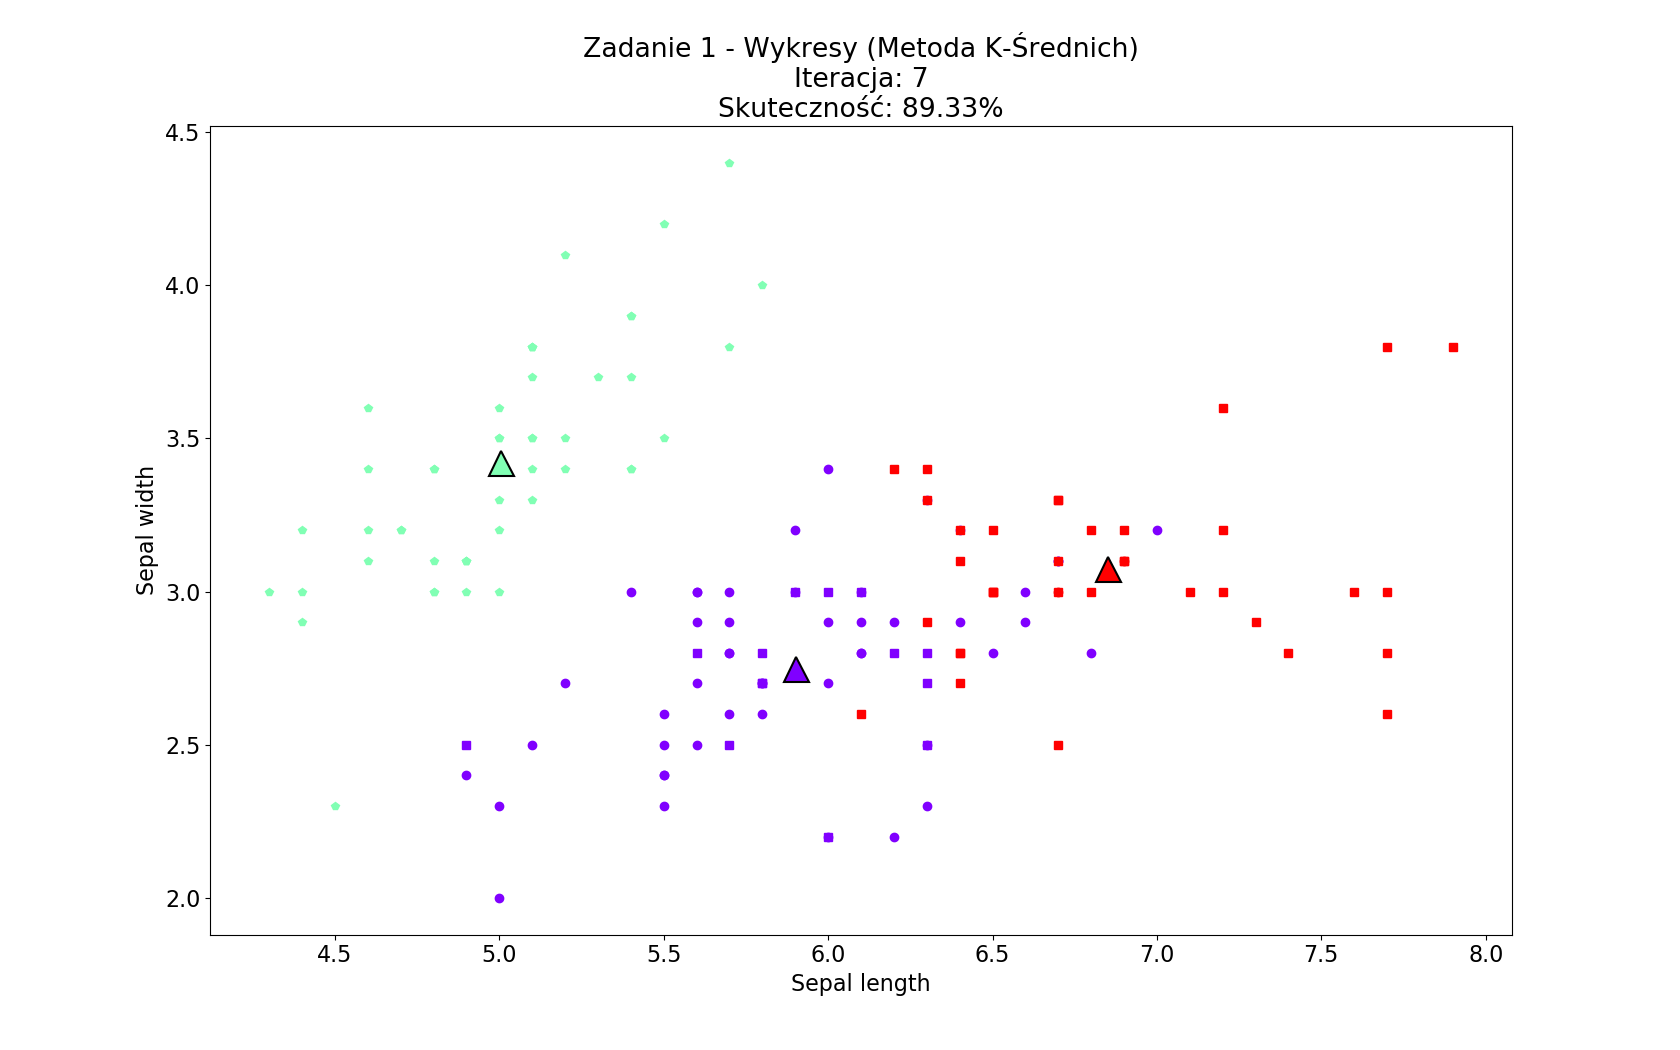
\includegraphics[width=\textwidth]{wykresy/plot_k_meansIrisDefault.png}
					\caption{Tryb domyślny danych}
				\end{figure}
			
				\begin{figure}[!htbp]
					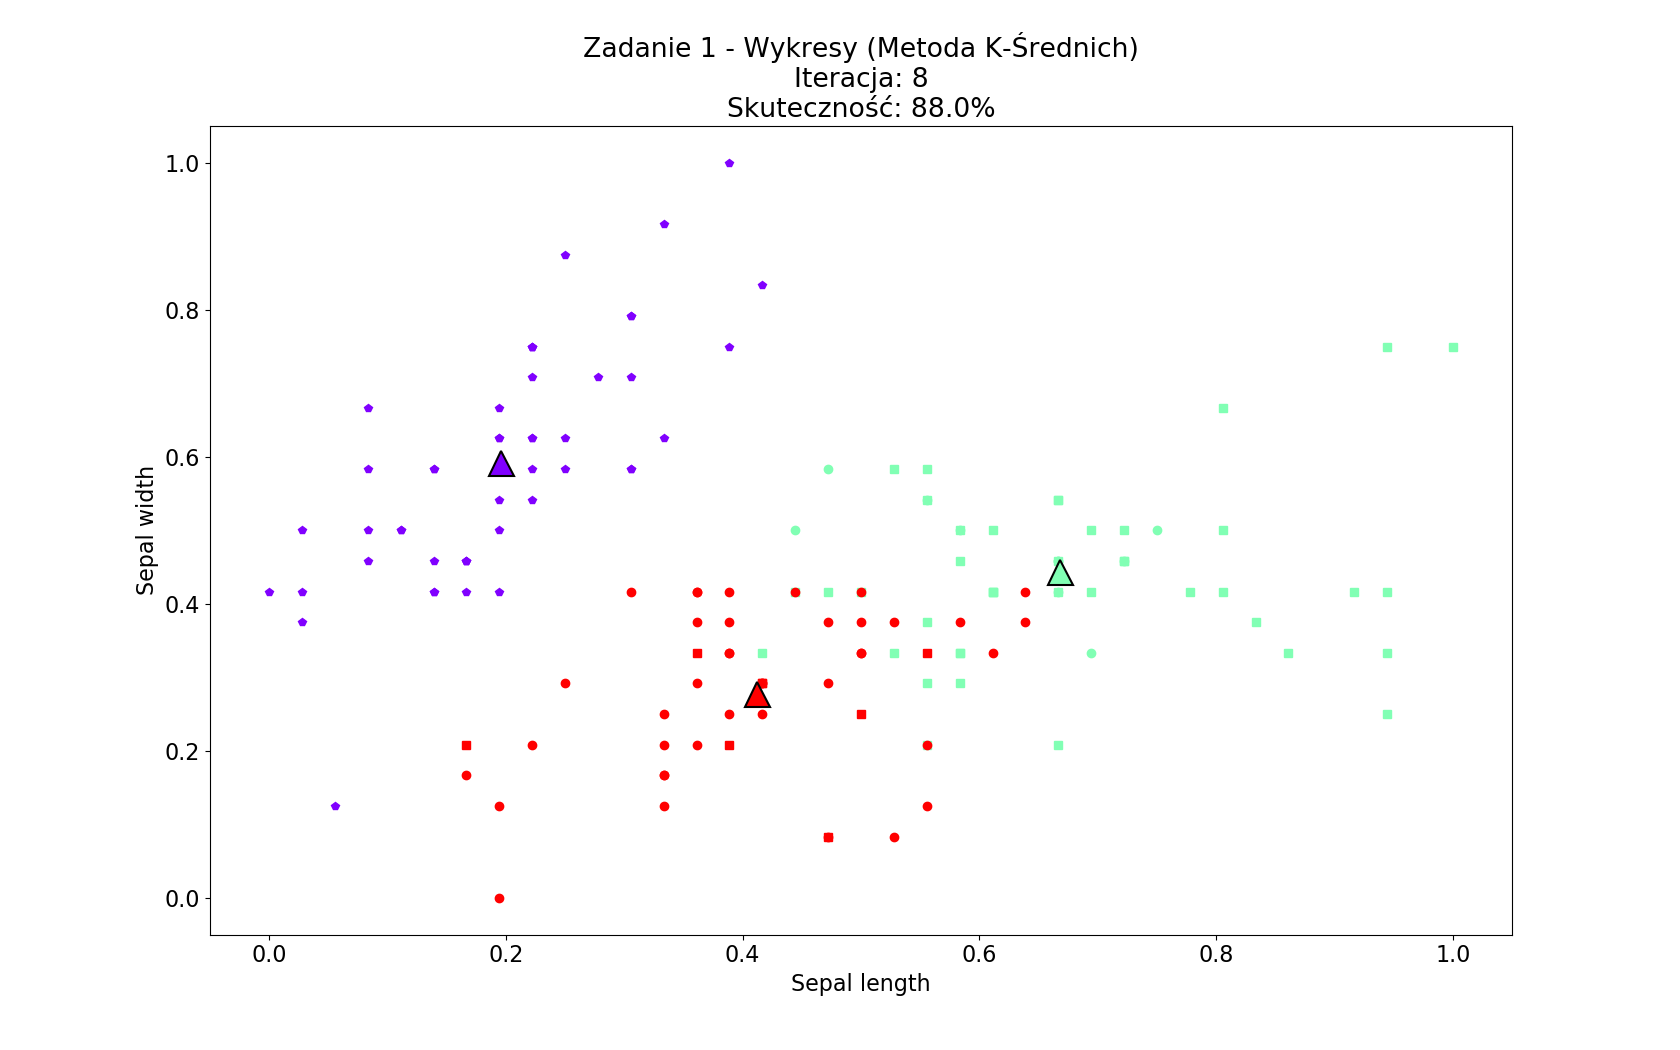
\includegraphics[width=\textwidth]{wykresy/plot_k_meansIrisNormalized.png}
					\caption{Tryb normalizacji danych}
				\end{figure}
		
				\begin{figure}[!htbp]
					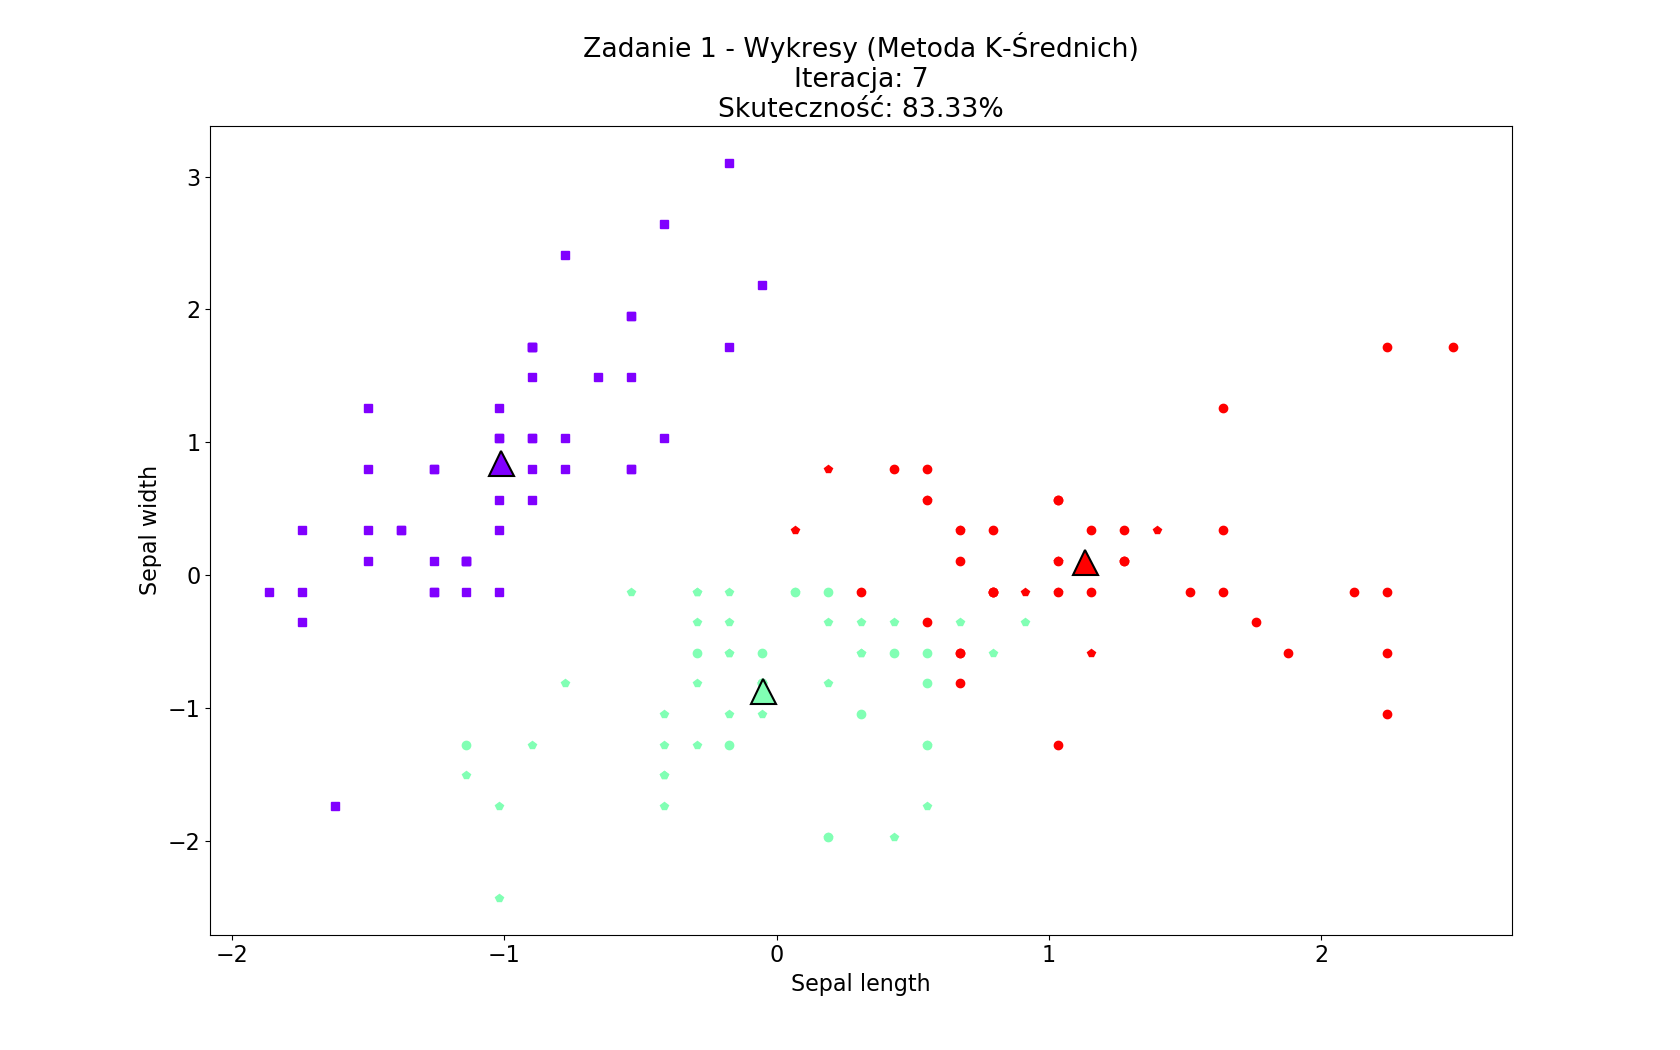
\includegraphics[width=\textwidth]{wykresy/plot_k_meansIrisStandadise.png}
					\caption{Tryb standaryzacji danych}
				\end{figure}
			\FloatBarrier
		}

		\subsubsection{Algorytm Kohonena}
		{ \iffalse
			Poniżej wykresy dla trzech trybów
				\begin{figure}[!htbp]
					\includegraphics[width=\textwidth]{wykresy/}
					\caption{Tryb domyślny danych}
				\end{figure}
			
				\begin{figure}[!htbp]
					\includegraphics[width=\textwidth]{wykresy/}
					\caption{Tryb normalizacji danych}
				\end{figure}
		
				\begin{figure}[!htbp]
					\includegraphics[width=\textwidth]{wykresy/}
					\caption{Tryb standaryzacji danych}
				\end{figure}
			\FloatBarrier
		\fi
		}

		\subsubsection{Algorytm gazu neuronowego}
		{
			\iffalse
			Poniżej wykresy dla trzech trybów
				\begin{figure}[!htbp]
					\includegraphics[width=\textwidth]{wykresy/}
					\caption{Tryb domyślny danych}
				\end{figure}
			
				\begin{figure}[!htbp]
					\includegraphics[width=\textwidth]{wykresy/}
					\caption{Tryb normalizacji danych}
				\end{figure}
		
				\begin{figure}[!htbp]
					\includegraphics[width=\textwidth]{wykresy/}
					\caption{Tryb standaryzacji danych}
				\end{figure}
			\FloatBarrier
		\fi
		}
	}
	\subsection{Zbiór win}
	{
		\subsubsection{Algorytm k - średnich}
		{
			Poniżej wykresy dla trzech trybów
				\begin{figure}[!htbp]
					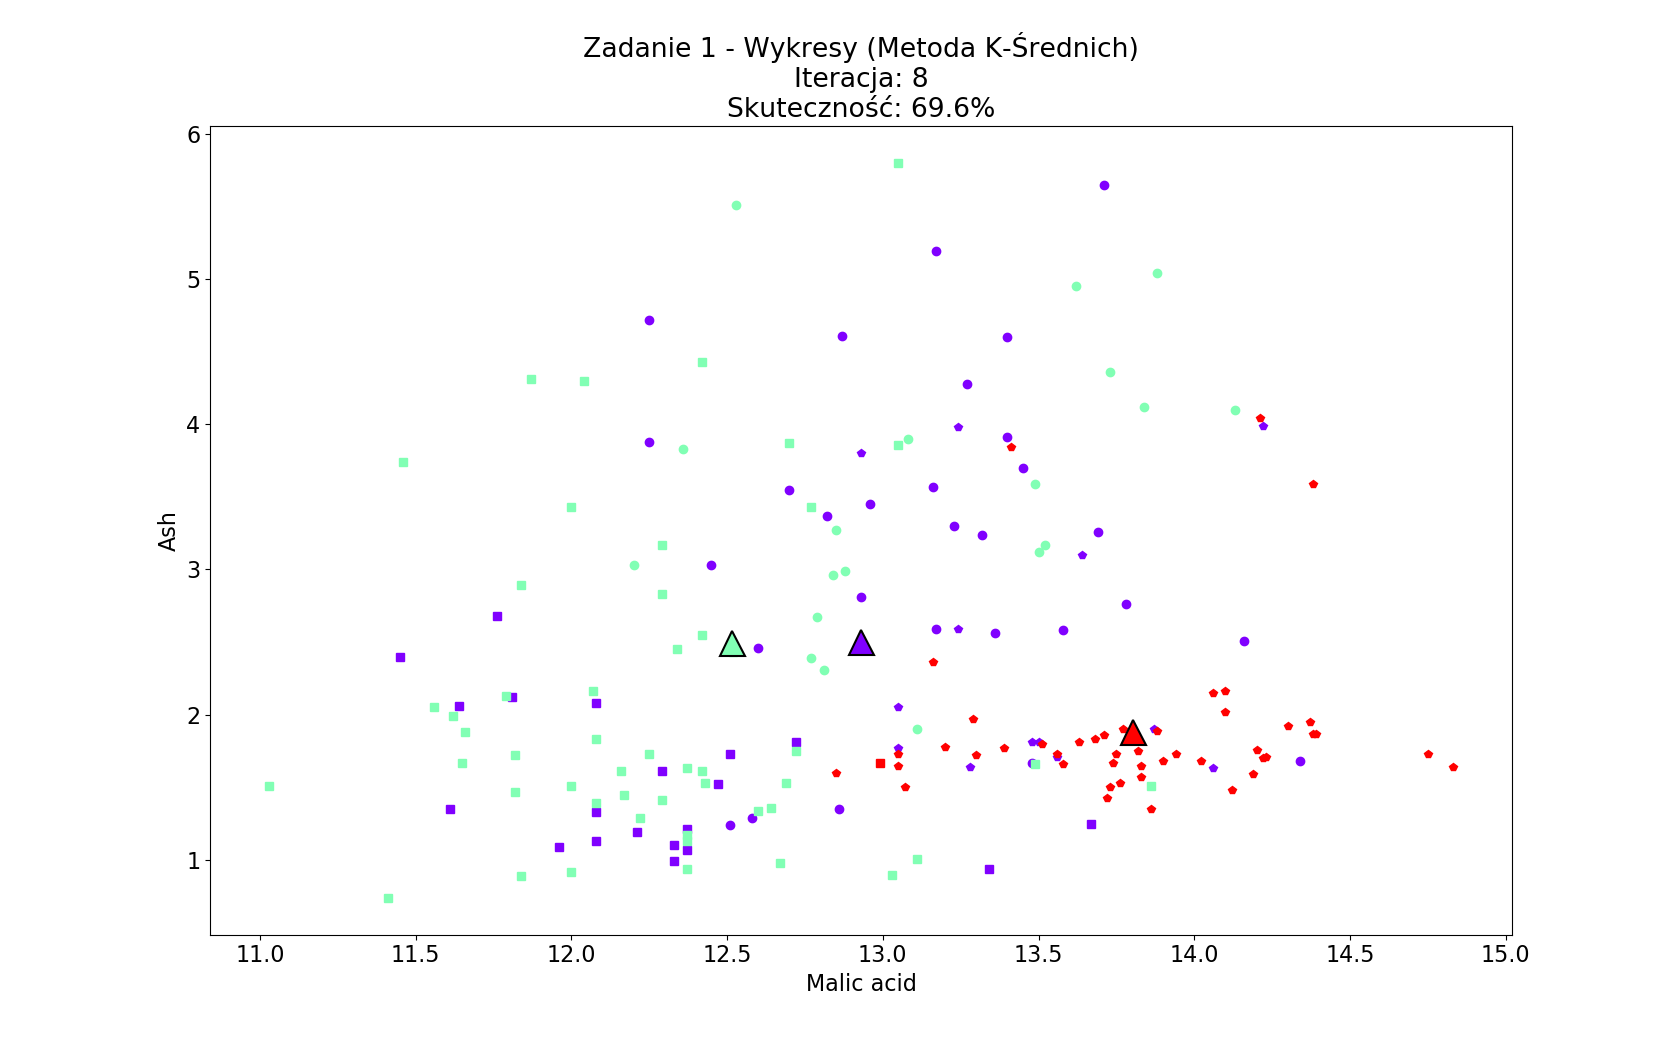
\includegraphics[width=\textwidth]{wykresy/plot_k_meansWineDefault.png}
					\caption{Tryb domyślny danych}
				\end{figure}
			
				\begin{figure}[!htbp]
					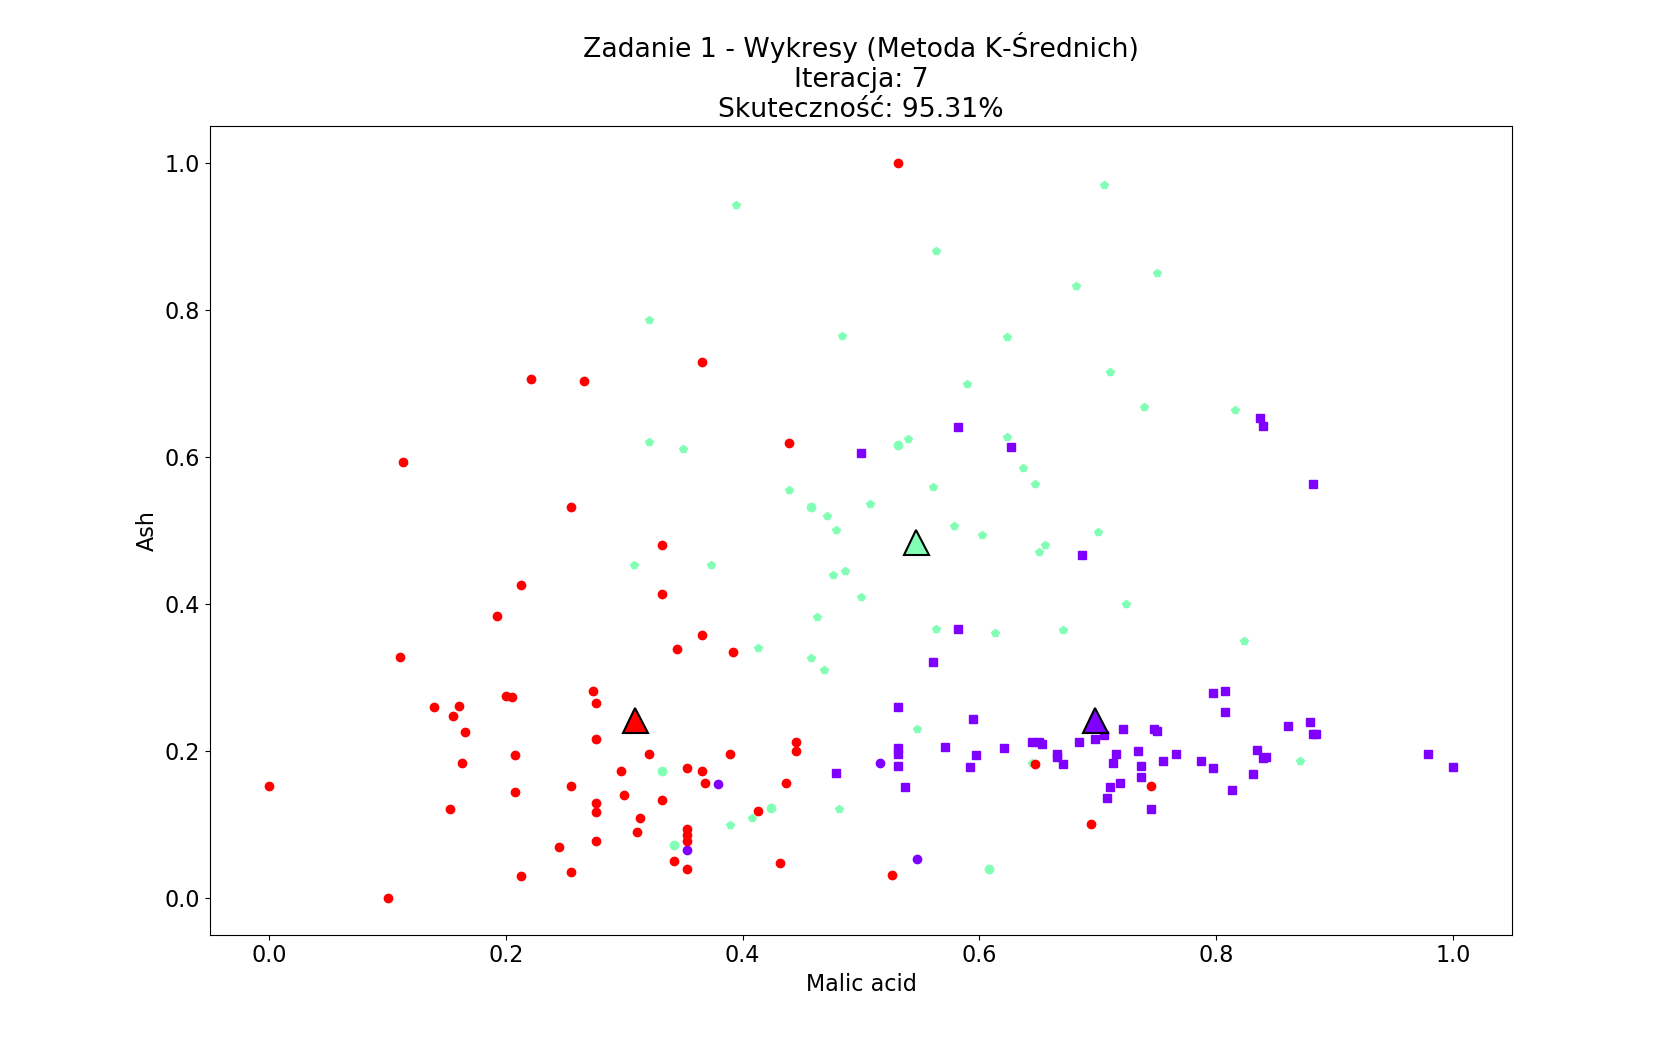
\includegraphics[width=\textwidth]{wykresy/plot_k_meansWineNormalised.png}
					\caption{Tryb normalizacji danych}
				\end{figure}
		
				\begin{figure}[!htbp]
					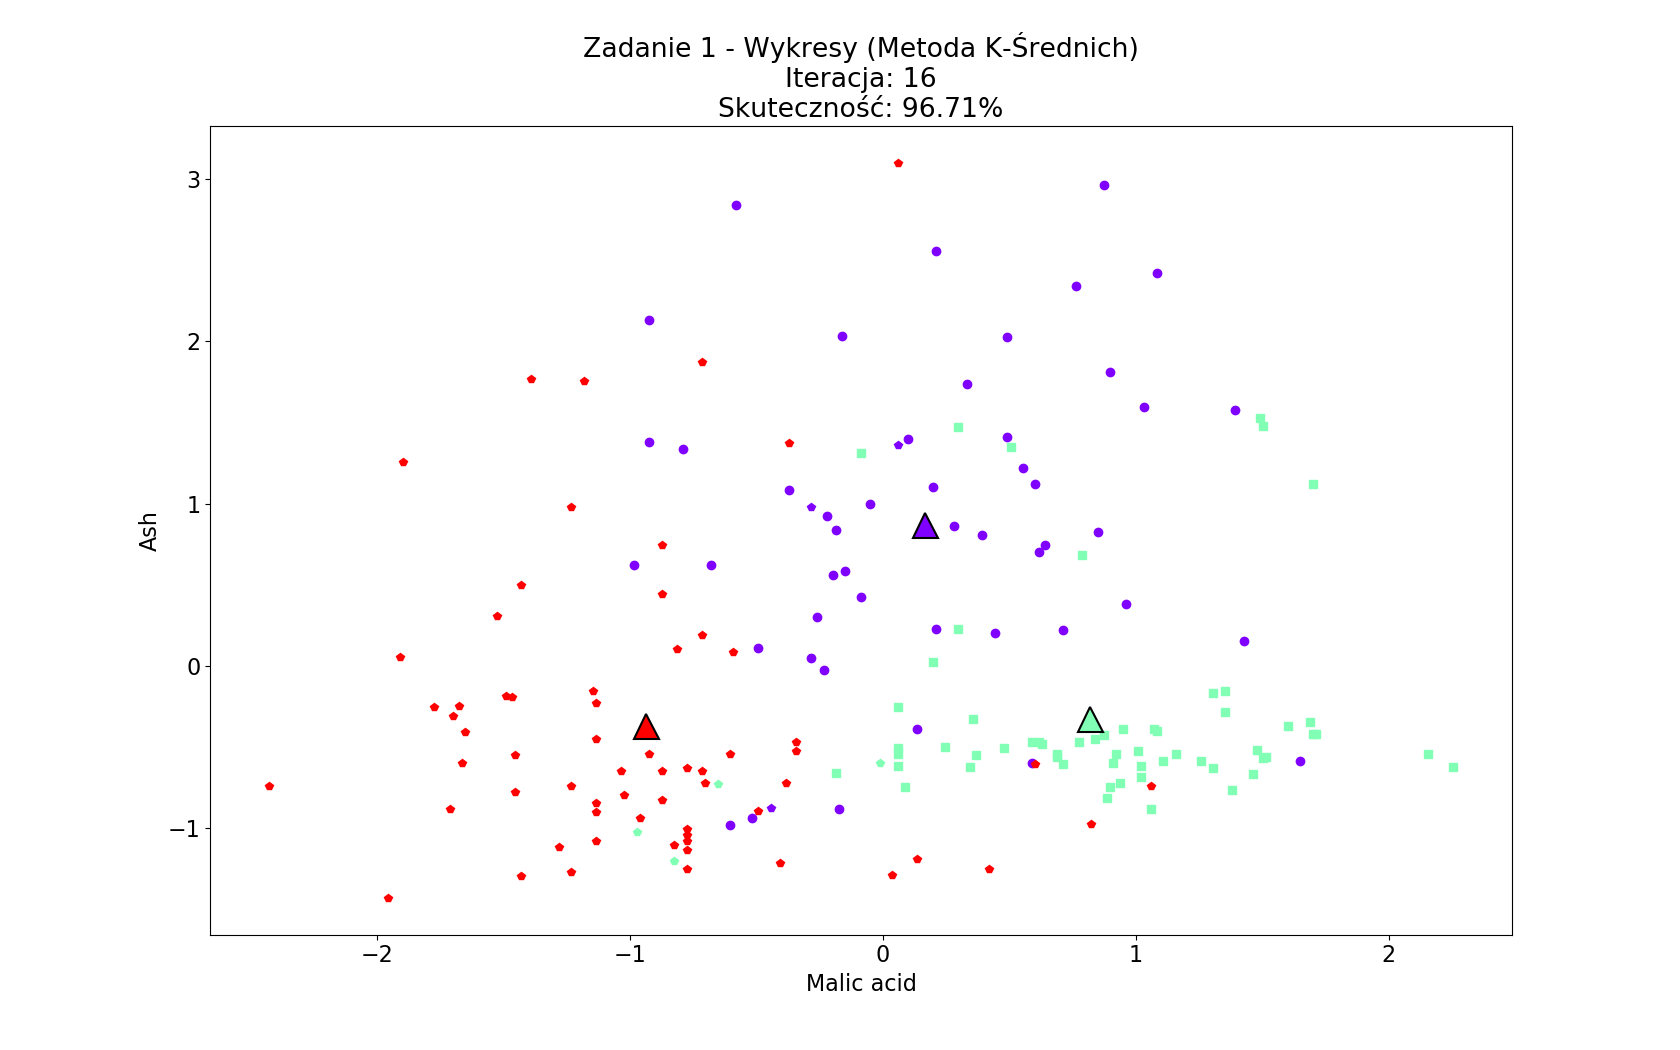
\includegraphics[width=\textwidth]{wykresy/plot_k_meansWineStandardise.png}
					\caption{Tryb standaryzacji danych}
				\end{figure}
			\FloatBarrier
		}

		\subsubsection{Algorytm Kohonena}
		{
			\iffalse
			Poniżej wykresy dla trzech trybów
				\begin{figure}[!htbp]
					\includegraphics[width=\textwidth]{wykresy/}
					\caption{Tryb domyślny danych}
				\end{figure}
			
				\begin{figure}[!htbp]
					\includegraphics[width=\textwidth]{wykresy/}
					\caption{Tryb normalizacji danych}
				\end{figure}
		
				\begin{figure}[!htbp]
					\includegraphics[width=\textwidth]{wykresy/}
					\caption{Tryb standaryzacji danych}
				\end{figure}
			\FloatBarrier
		\fi
		}

		\subsubsection{Algorytm gazu neuronowego}
		{
			\iffalse
			Poniżej wykresy dla trzech trybów
				\begin{figure}[!htbp]
					\includegraphics[width=\textwidth]{wykresy/}
					\caption{Tryb domyślny danych}
				\end{figure}
			
				\begin{figure}[!htbp]
					\includegraphics[width=\textwidth]{wykresy/}
					\caption{Tryb normalizacji danych}
				\end{figure}
		
				\begin{figure}[!htbp]
					\includegraphics[width=\textwidth]{wykresy/}
					\caption{Tryb standaryzacji danych}
				\end{figure}
			\FloatBarrier
		\fi
		}
	}
	\subsection{Zbiór abalone}
	{
		\subsubsection{Algorytm k - średnich}
		{
			Poniżej wykresy dla trzech trybów
				\begin{figure}[!htbp]
					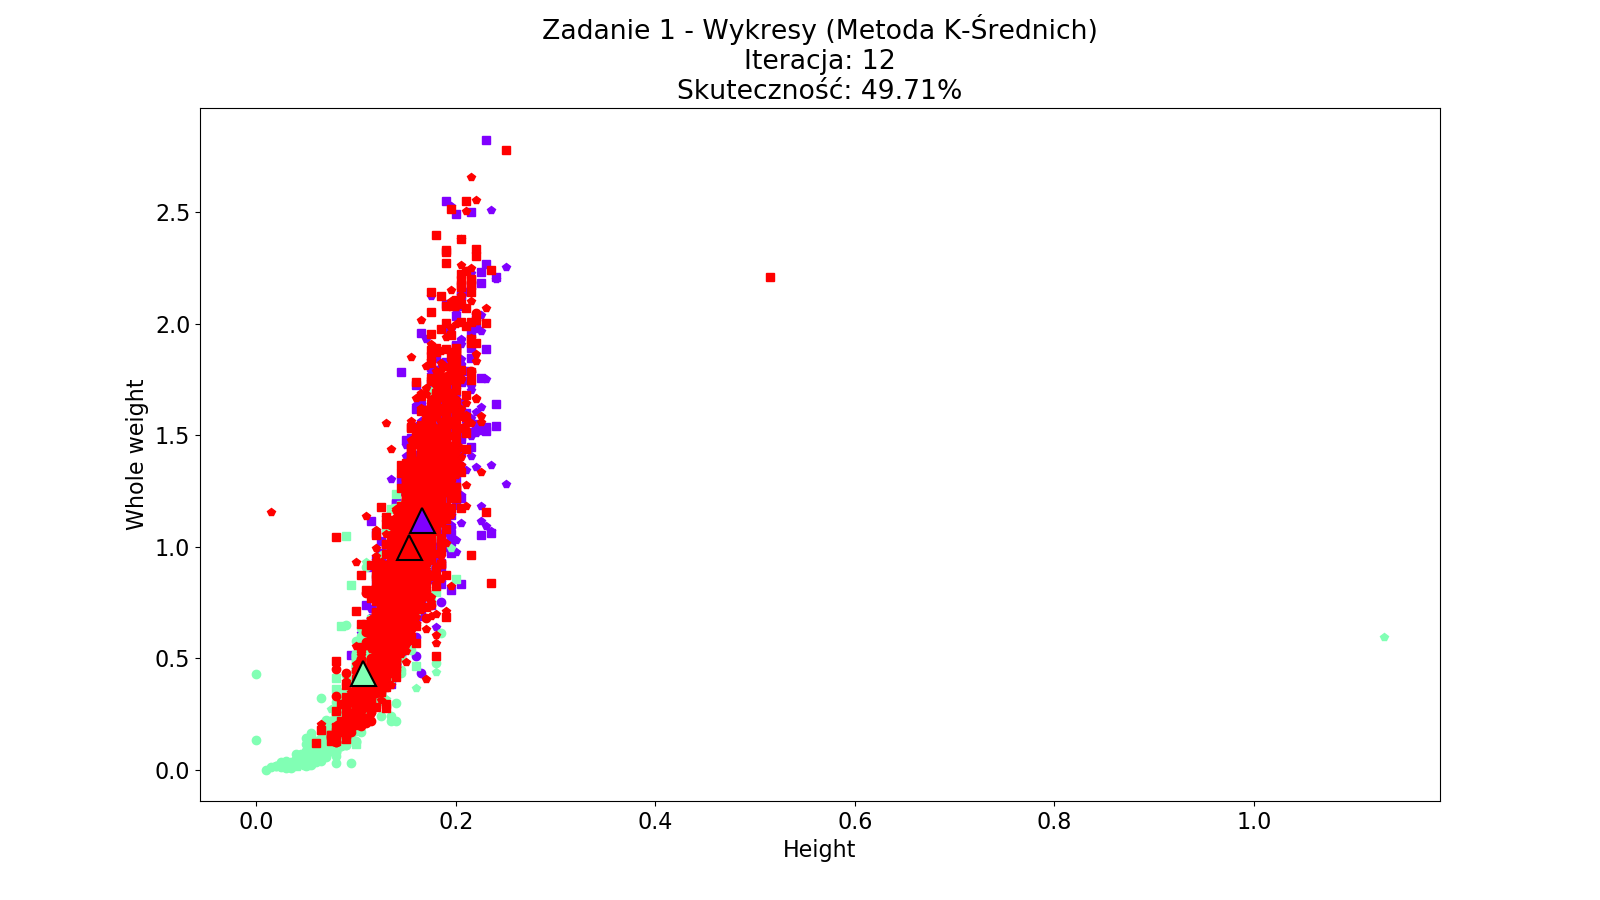
\includegraphics[width=\textwidth]{wykresy/plot_k_meansAbaloneDefault.png}
					\caption{Tryb domyślny danych}
				\end{figure}
			
				\begin{figure}[!htbp]
					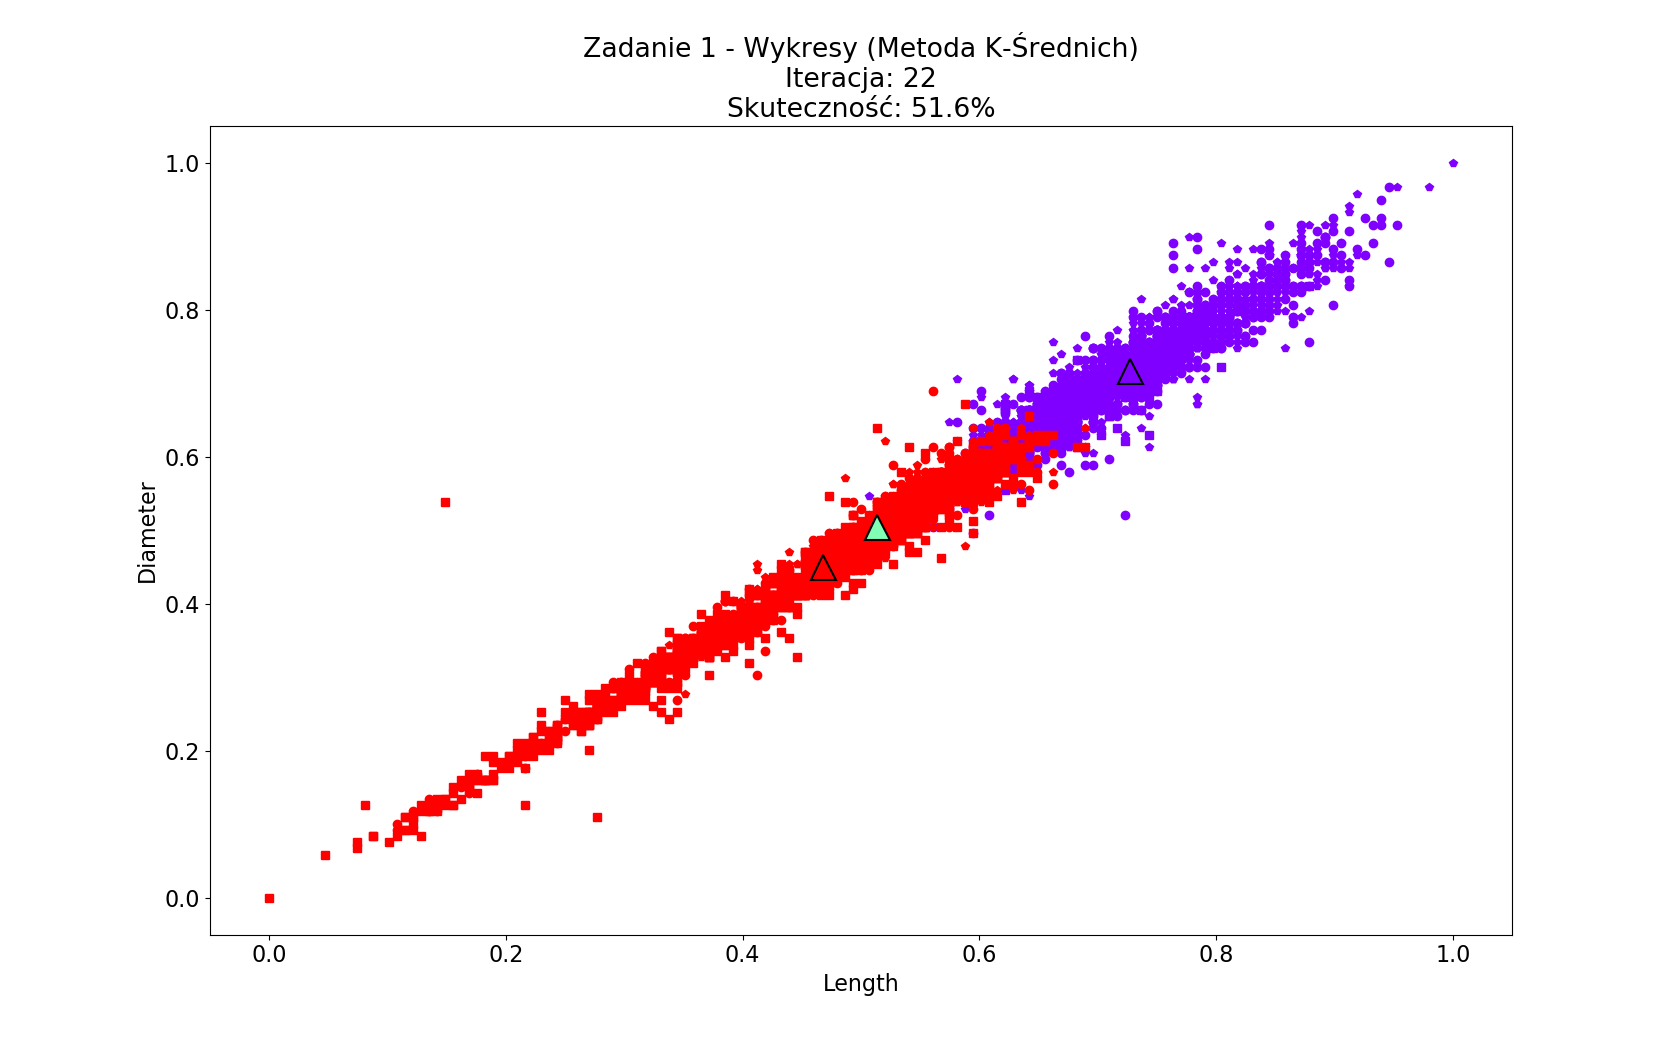
\includegraphics[width=\textwidth]{wykresy/plot_k_meansAbaloneNormalised.png}
					\caption{Tryb normalizacji danych}
				\end{figure}
		
				\begin{figure}[!htbp]
					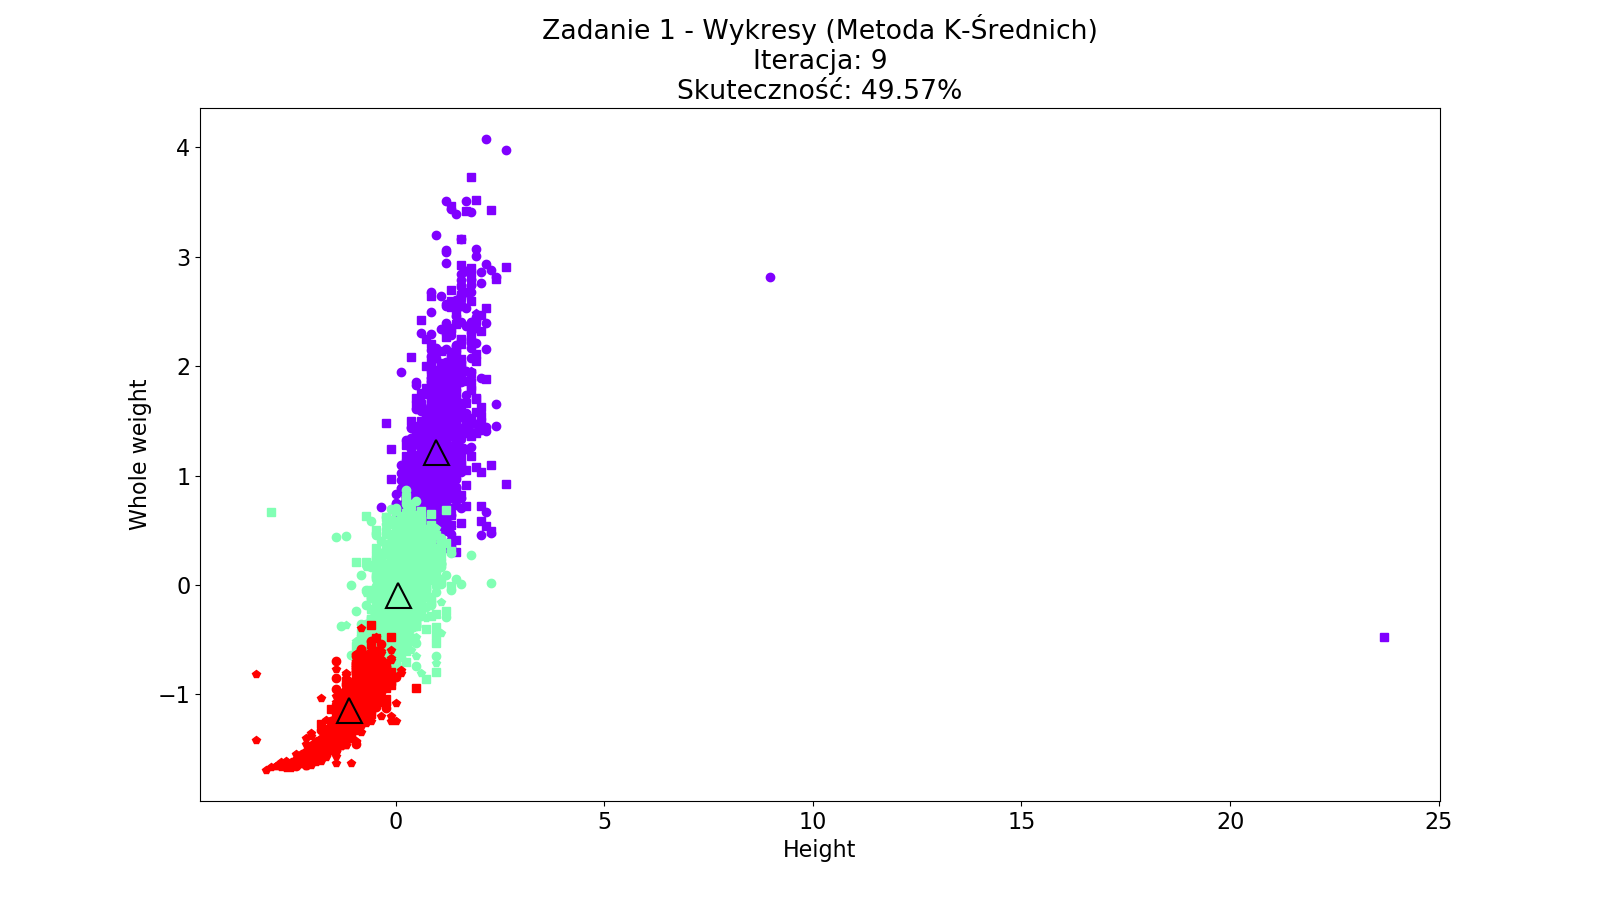
\includegraphics[width=\textwidth]{wykresy/plot_k_meansAbaloneStandardise.png}
					\caption{Tryb standaryzacji danych}
				\end{figure}
			\FloatBarrier
		}

		\subsubsection{Algorytm Kohonena}
		{
			\iffalse
			Poniżej wykresy dla trzech trybów
				\begin{figure}[!htbp]
					\includegraphics[width=\textwidth]{wykresy/}
					\caption{Tryb domyślny danych}
				\end{figure}
			
				\begin{figure}[!htbp]
					\includegraphics[width=\textwidth]{wykresy/}
					\caption{Tryb normalizacji danych}
				\end{figure}
		
				\begin{figure}[!htbp]
					\includegraphics[width=\textwidth]{wykresy/}
					\caption{Tryb standaryzacji danych}
				\end{figure}
			\FloatBarrier
		\fi
		}

		\subsubsection{Algorytm gazu neuronowego}
		{
			\iffalse
			Poniżej wykresy dla trzech trybów
				\begin{figure}[!htbp]
					\includegraphics[width=\textwidth]{wykresy/}
					\caption{Tryb domyślny danych}
				\end{figure}
			
				\begin{figure}[!htbp]
					\includegraphics[width=\textwidth]{wykresy/}
					\caption{Tryb normalizacji danych}
				\end{figure}
		
				\begin{figure}[!htbp]
					\includegraphics[width=\textwidth]{wykresy/}
					\caption{Tryb standaryzacji danych}
				\end{figure}
			\FloatBarrier
		\fi
		}
	}
}

\section{Dyskusja}
{
	Na podstawie uzyskanych wyników stwierdzamy, że
}

\section{Wnioski}
{
	Podsumowując wykonane zadanie wnioskujemy, że:\\
}

\begin{thebibliography}{0}
  \bibitem{l2short}\url{ http://wikizmsi.zut.edu.pl/uploads/6/6f/InstrukcjaGaz.pdf}
  \bibitem{l2short} \url{https://en.wikipedia.org/wiki/K-means\_clustering}
  \bibitem{l2short} \url{http://www.michalbereta.pl/dydaktyka/WdoSI/lab_neuronowe_II}
  \bibitem{l2short} 
\end{thebibliography}

{

}

\end{document}
